\chapter{Progettazione concettuale}
    \section{Class Diagram}

    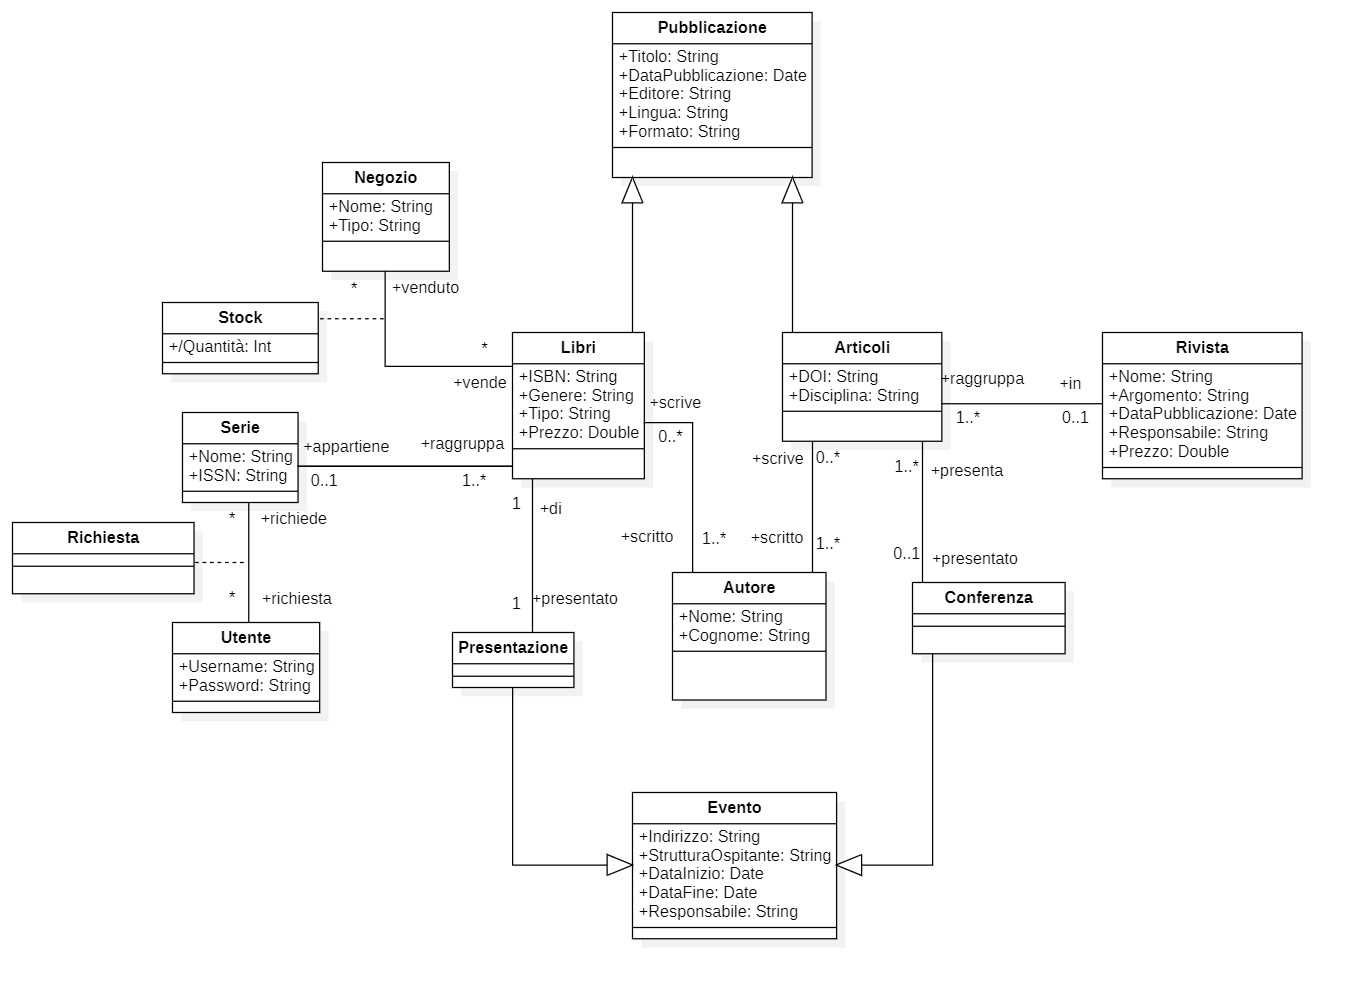
\includegraphics[scale=0.3]{Immagini/SchemaConcettuale.png}
        
    \section{Analisi della ristrutturazione del Class Diagram}
        In questa fase verranno effettuate delle modifiche che renderanno il Class Diagram
        più adatto a una traduzione al modello logico \textcolor{red}{(magari scriviamo meglio sta parte)}
        \subsection{Analisi delle ridondanze}
        Nel Diagramma Concettuale non ci sono ridondanze tali da essere eliminate.
        \subsection{Analisi degli identificativi}
        In questa fase andremo a scegliere uno o più attributi atti a identificare univocamente
        le varie entità presenti nello schema precedente, in particolare:
            \begin{enumerate}
            \item L'entità \textbf{Libro} presenta l'attributo ISBN che rappresenta una possibile chiave primaria,
                  tuttavia è stato scelto di aggiungere un attributo \textit{ID\_Libro} in modo tale da aumentare
                  la velocità di accesso agli indici.
            \item Per \textbf{Articolo scientifico} la situazione è analoga, è stato quindi aggiunto un attributo
                  \textit{ID\_Articolo}.
            \item Nel caso dell'entità \textbf{Rivista}, la quale presenta un attributo ISSN che è chiave candidata,
                  di inserire un ulteriore attributo \textit{ID\_Rivista}.
            \item Sarebbe possibile identificare un \textbf{Evento} tramite un insieme piuttosto ampio di attributi, è
                  stato quindi aggiunto un attributo \textit{ID\_Evento}.
            \item Dato che diversi \textbf{Autori} potrebbero avere lo stesso nome, è stato aggiunto l'identificativo
                  \textit{ID\_Autore}.
            \item Dato che l'entità \textbf{Negozio} non presenta alcuna chiave candidata, è stato aggiunto l'attributo
                  \textit{ID\_Negozio}.
            \item \'E stato deciso di aggiungere a \textbf{Serie} un attributo \textit{ID\_Serie} per ridurre il volume degli
                  indici associati.
            \end{enumerate}
        \subsection{Rimozione degli attributi multivalore}
            Non sono presenti attributi multivalore.
        \subsection{Rimozione degli attributi composti}
            Non sono presenti attributi composti.
        \subsection{Partizione/Accorpamento delle associazioni}
            
        \subsection{Rimozione delle gerarchie}
            In questo diagramma sono presenti 2 generalizzazioni e 4 relative specializzazioni.
            In particolare:

            Per quanto riguarda la generalizzazione \textbf{Pubblicazione}, si è scelto di accorpare l'entità padre
            nelle entità figlie, ottenendo come risultato:
            \begin{itemize}
                  \item Una entità \textbf{Libro} aventi tutti gli attributi di \textbf{Pubblicazione} più
                        gli attributi della precedente entità \textbf{Libro}.
                  \item Analogamente, l'entità \textbf{Articolo} avrà come attributi, quelli di \textbf{Pubblicazione}
                        uniti agli attributi di \textbf{Articolo}.
            \end{itemize}
    
    \section{Class Diagram ristrutturato}
    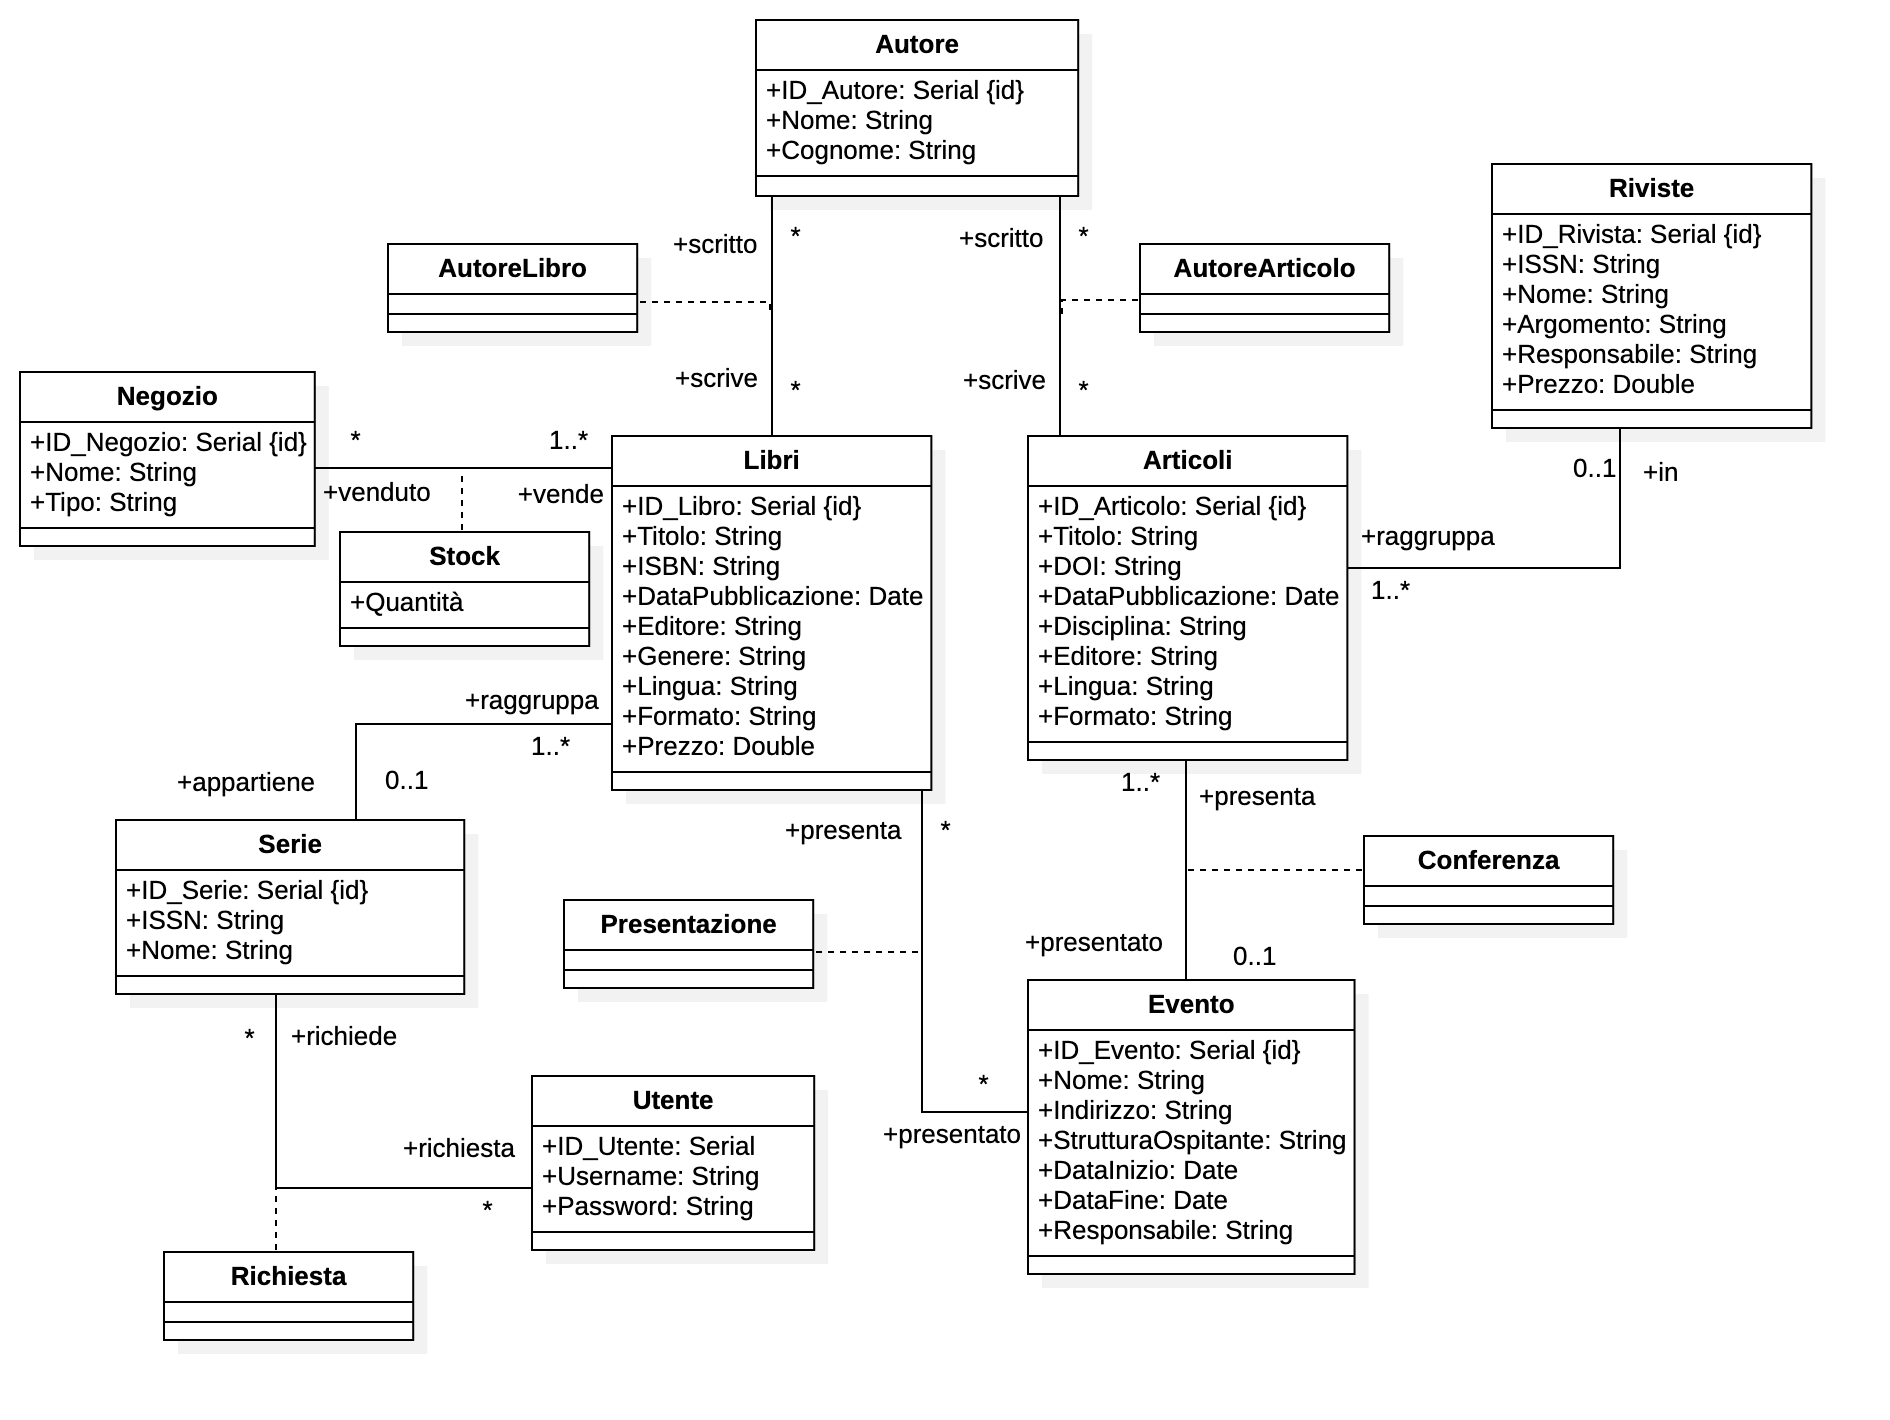
\includegraphics[scale=0.25]{Immagini/SchemaRistrutturato.png}
    \pagebreak
    \section{Dizionario delle classi}

\begin{table}[]
      \begin{longtable}{@{}lll@{}}
      \toprule
      \multicolumn{1}{|l|}{Classe}           & \multicolumn{1}{l|}{Attributi}                                                                                                                            & \multicolumn{1}{l|}{Descrizione}                                                                                                                                                              \\ \midrule
      \multicolumn{1}{|l|}{Articolo}         & \multicolumn{1}{l|}{\begin{tabular}[c]{@{}l@{}}ID\_Articolo\\ Titolo\\ Doi\\ DataPubblicazione\\ Editore\\ Lingua\\ Formato\end{tabular}}                 & \multicolumn{1}{l|}{\begin{tabular}[c]{@{}l@{}}Classe che conserva le \\ informazioni relative\\ agli articoli presenti\\ nel sistema\end{tabular}}                                           \\ \midrule
      \multicolumn{1}{|l|}{Autore}           & \multicolumn{1}{l|}{\begin{tabular}[c]{@{}l@{}}ID\_Autore\\ Nome\\ Cognome\end{tabular}}                                                                  & \multicolumn{1}{l|}{\begin{tabular}[c]{@{}l@{}}Classe che conserva le\\ informazioni relative\\ agli autori presenti\\ nel sistema\end{tabular}}                                              \\ \midrule
      \multicolumn{1}{|l|}{Rivista}          & \multicolumn{1}{l|}{\begin{tabular}[c]{@{}l@{}}ID\_Rivista\\ ISSN\\ Nome\\ Argomento\\ DataPubblicazione\\ Responsabile\end{tabular}}                     & \multicolumn{1}{l|}{\begin{tabular}[c]{@{}l@{}}Classe che conserva le\\ informazioni relative\\ alle riviste scientifiche\\ presenti nel sistema\end{tabular}}                                \\ \midrule
      \multicolumn{1}{|l|}{AutoreArticolo}   & \multicolumn{1}{l|}{\begin{tabular}[c]{@{}l@{}}Autore\\ Articolo\end{tabular}}                                                                            & \multicolumn{1}{l|}{\begin{tabular}[c]{@{}l@{}}Classe che conserva\\ le informazioni sugli\\ autori degli articoli\\ scientifici\end{tabular}}                                                \\ \midrule
      \multicolumn{1}{|l|}{ArticolInRivista} & \multicolumn{1}{l|}{\begin{tabular}[c]{@{}l@{}}Rivista\\ Articolo\end{tabular}}                                                                           & \multicolumn{1}{l|}{\begin{tabular}[c]{@{}l@{}}Classe che mette in\\ relazione Articoli\\ e Riviste a cui\\ i primi appartengono\end{tabular}}                                                \\ \midrule
      \multicolumn{1}{|l|}{Evento}           & \multicolumn{1}{l|}{\begin{tabular}[c]{@{}l@{}}ID\_Evento\\ Indirizzo\\ StrutturaOspitante\\ DataInizio\\ DataFine\\ Responsabile\end{tabular}}           & \multicolumn{1}{l|}{\begin{tabular}[c]{@{}l@{}}Classe che conserva le\\ informazioni sugli \\ eventi relativi a \\ presentazioni di libri\\ oppure a conferenze \\ scientifiche\end{tabular}} \\ \midrule
      \multicolumn{1}{|l|}{Conferenza}       & \multicolumn{1}{l|}{\begin{tabular}[c]{@{}l@{}}Evento\\ Articolo\end{tabular}}                                                                            & \multicolumn{1}{l|}{\begin{tabular}[c]{@{}l@{}}Classe che mette in\\ relazione eventi e\\ articoli scientifici\end{tabular}}                                                                  \\ \midrule
      \multicolumn{1}{|l|}{Libro}            & \multicolumn{1}{l|}{\begin{tabular}[c]{@{}l@{}}ID\_Libro\\ Titolo\\ ISBN\\ DataPubblicazione\\ Editore\\ Genere\\ Lingua\\ Formato\\ Prezzo\end{tabular}} & \multicolumn{1}{l|}{\begin{tabular}[c]{@{}l@{}}Classe che conserva\\ le principali \\ informazioni sui libri\\ presenti nel sistema\end{tabular}}                                             \\ \midrule
      \multicolumn{1}{|l|}{AutoreLibro}      & \multicolumn{1}{l|}{\begin{tabular}[c]{@{}l@{}}Autore\\ Libro\end{tabular}}                                                                               & \multicolumn{1}{l|}{\begin{tabular}[c]{@{}l@{}}Classe che mette in\\ relazione Autori e Libri\end{tabular}}                                                                                   \\ \midrule
      \multicolumn{1}{|l|}{Presentazione}    & \multicolumn{1}{l|}{\begin{tabular}[c]{@{}l@{}}Evento\\ Libro\end{tabular}}                                                                               & \multicolumn{1}{l|}{\begin{tabular}[c]{@{}l@{}}Classe che conserva\\ le informazioni relative\\ a presentazioni di libri\end{tabular}}                                                        \\ \midrule
      \multicolumn{1}{|l|}{Serie}            & \multicolumn{1}{l|}{\begin{tabular}[c]{@{}l@{}}ID\_Serie\\ ISSN\\ Nome\end{tabular}}                                                                      & \multicolumn{1}{l|}{\begin{tabular}[c]{@{}l@{}}Classe che conserva\\ le informazioni relative\\ alle Serie di libri\end{tabular}}                                                             \\ \midrule
      \multicolumn{1}{|l|}{LibroInSerie}     & \multicolumn{1}{l|}{\begin{tabular}[c]{@{}l@{}}ID\_Serie\\ Libro\\ LibroSuccessivo\end{tabular}}                                                          & \multicolumn{1}{l|}{\begin{tabular}[c]{@{}l@{}}Classe che mette in\\ relazione Serie, Libri\\ e relativi sequel\end{tabular}}                                                                 \\ \midrule
      \multicolumn{1}{|l|}{Negozio}          & \multicolumn{1}{l|}{\begin{tabular}[c]{@{}l@{}}ID\_Negozio\\ Nome\\ Tipo\end{tabular}}                                                                    & \multicolumn{1}{l|}{\begin{tabular}[c]{@{}l@{}}Classe che conserva\\ le informazioni\\ relative ai Negozi presenti\\ nel sistema\end{tabular}}                                                \\ \midrule
      \multicolumn{1}{|l|}{Stock}            & \multicolumn{1}{l|}{\begin{tabular}[c]{@{}l@{}}Negozio\\ Libro\end{tabular}}                                                                              & \multicolumn{1}{l|}{\begin{tabular}[c]{@{}l@{}}Classe che conserva le\\ informazioni relative ai\\ libri acquistabili da\\ determinati negozi\end{tabular}}                                   \\ \midrule
      \multicolumn{1}{|l|}{Utente}           & \multicolumn{1}{l|}{\begin{tabular}[c]{@{}l@{}}ID\_Utente\\ Username\\ Password\end{tabular}}                                                             & \multicolumn{1}{l|}{\begin{tabular}[c]{@{}l@{}}Classe che conserva le\\ informazioni relative\\ agli Utenti registrati sul\\ sistema\end{tabular}}                                            \\ \midrule
      \multicolumn{1}{|l|}{Richiesta}        & \multicolumn{1}{l|}{\begin{tabular}[c]{@{}l@{}}Utente\\ Serie\\ Disponibilità\end{tabular}}                                                               & \multicolumn{1}{l|}{\begin{tabular}[c]{@{}l@{}}Classe che gestisce le\\ richieste fatte dagli utenti\\ relativamente alle\\ disponibilità di libri\end{tabular}}                              \\ \midrule
                                             &                                                                                                                                                           &                                                                                                                                                                                               \\
                                             &                                                                                                                                                           &                                                                                                                                                                                               \\
                                             &                                                                                                                                                           &                                                                                                                                                                                              
      \end{longtable}
      \end{table}
    \section{Dizionario delle associazioni}